\chapter{Introduction}
\label{cha:intro}
\Acrfullpl{WSN} enable scientists to monitor active volcanoes without having to risk their lives when they need seismic measurements \cite{reventador}, make homes smarter by connecting all appliances together \cite{chan-smart-home-review} and will allow future energy production to be tuned to the real-time energy demand of consumers \cite{gungor-smart-grid-technologies} \cite{gungor-smart-grid-survey}. However, \glspl{WSN} need to evolve in order to last for many years, and thus operators must be able to distribute updates to nodes in these networks \cite{han-sensor-update-survey} \cite{wang-reprogramming}. Since these nodes are very resource-constrained and often battery-powered (e.g. AVR Zigduino \cite{zigduino-manual}, TMote Sky \cite{tmote-sky-manual}), the distribution of such large update files must be done in an efficient but fast manner.

This master's thesis presents NanoTorrent as a \acrfull{P2P} file distribution protocol aimed at \glspl{WSN}. The problem context is described in section \ref{sec:intro:context}, going in-depth about the \acrlong{IoT} and \acrlongpl{WSN} and explaining \acrlong{P2P} architectures. Section \ref{sec:intro:problem} discusses the problem and challenges imposed by \glspl{WSN}. Section \ref{sec:intro:contrib} sketches the contributions of the proposed solution. Finally, section \ref{sec:intro:structure} outlines the structure of the text.

\section{Problem context}
\label{sec:intro:context}

\subsection{Internet of Things}
\label{sec:intro:iot}
The \acrfull{IoT} is a vision where many small embedded electronic devices are deployed in a physical environment to monitor their environment and communicate with each other and the outside world to achieve certain goals \cite{iotcluster15}. In the research context for \gls{IoT}, the challenge is to make the physical world `smart': physical objects become connected to the Internet and can be monitored or operated from anywhere at any time. In other words, bringing the world of `things' to the digital world of the Internet, as shown in figure \ref{fig:intro:iot:framework}.

\begin{figure}
    \centering
    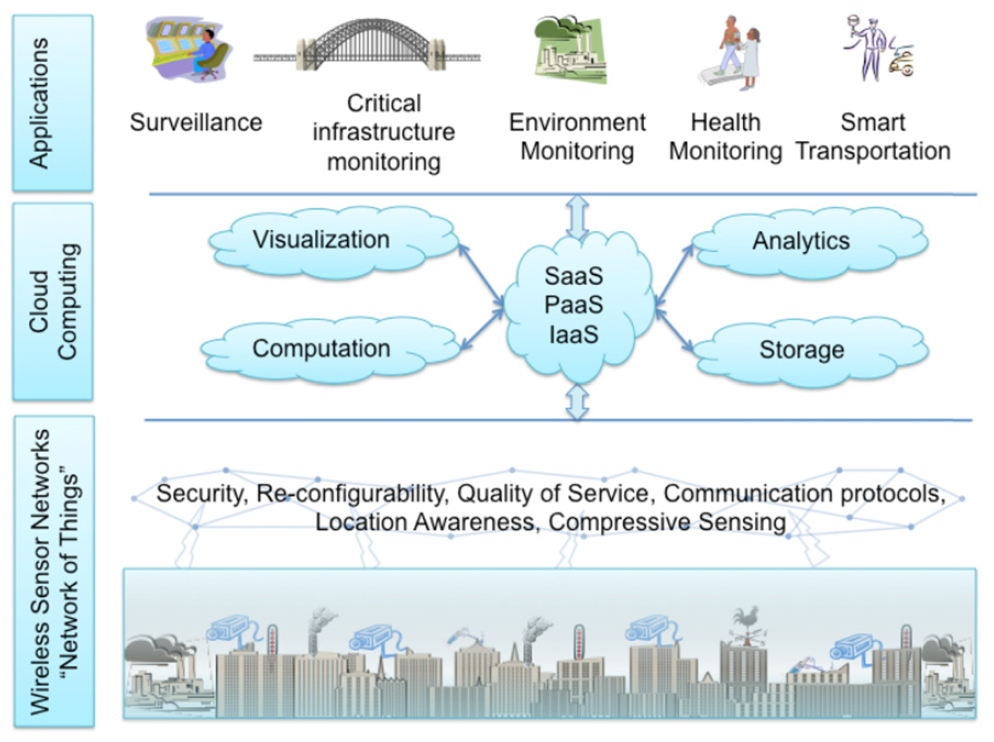
\includegraphics[width=\textwidth]{images/gubbi-iot-framework.png}
    \caption[Conceptual framework for IoT applications]{A conceptual framework for \gls{IoT} applications, integrating the world of `things' (in \glspl{WSN}) with the digital world of the Internet. \cite{gubbi-iot-vision}}
    \label{fig:intro:iot:framework}
\end{figure}

In order to integrate such a large number of devices into the global Internet infrastructure, \gls{IoT} devices use \gls{IPv6} for networking. The \gls{IPv6} address space allows for $2^{128}$ possible addresses, which is more than plenty to support the rapid growth of these devices. The same technologies that power the Internet are adapted to the scale of \gls{IoT} devices, such that they can communicate with outside networks in a uniform and transparent manner. For example, \gls{IoT} devices can send and receive \gls{IPv6} packets, download a file from a website, or even host a small web server.

The (possible) applications for \gls{IoT} encompass nearly all fields, ranging from improving comfort at your own house to controlling critical wide-range infrastructures:
\begin{description}
\item[Smart homes.] By connecting household appliances, temperature sensors and security cameras to the Internet, a house owner could control his living comfort from any device at any time \cite{chan-smart-home-review}. Instead of having to deal with many different switches and remotes around his house, he could have a single dashboard to monitor and control all of his devices. Such a dashboard could also allow for combined actions with multiple devices, for example activating the air conditioning also automatically closes the window blinds and the room doors.
\item[Smart energy grids.] With the shift from fossil resources to renewable resources, energy production is becoming more volatile and less predictable. Whereas coal and nuclear power plants can produce electricity at any time, the energy output of solar and wind plants depends on the time and weather conditions. This can lead to shortages or blackouts during calm cloudy days, or oversupply on windy sunny days. To deal with these fluctuations, smart energy grids should have the capability of predicting consumption behaviour on a more fine-grained basis, and shifting consumption peaks to better match production capacity  \cite{gungor-smart-grid-survey}. For example, houses could be fitted with smart meters which continuously measure electricity consumption and report frequently to the energy producers so they can make better predictions. Smart washing machines could also be programmed to activate when the energy demand is low, in order to shift consumption peaks. These meters and appliances need to communicate with each other and with the rest of the energy grid, posing many \gls{IT} challenges for the supporting \gls{IT} architectures and technologies \cite{gungor-smart-grid-technologies}, shown in figure \ref{fig:intro:iot:smart-grid}.
\item[Earthquake and volcano monitoring.] To protect people living in seismically active regions such as fault lines and volcanoes, scientists must be able to predict future earthquakes or eruptions so people can be evacuated in time. Improving these predictions requires more frequent and accurate seismic measurements. However, sending humans into the field to measure seismic activity is dangerous. Instead, a network of monitoring devices can be deployed to collect measurements and report back to a base station \cite{reventador} (illustrated in figure \ref{fig:intro:iot:reventador}). These devices can make more frequent measurements, and can be deployed in more dangerous places where it is unsafe for humans (e.g. inside the crater of a volcano).
\end{description}

\begin{figure}
    \centering
    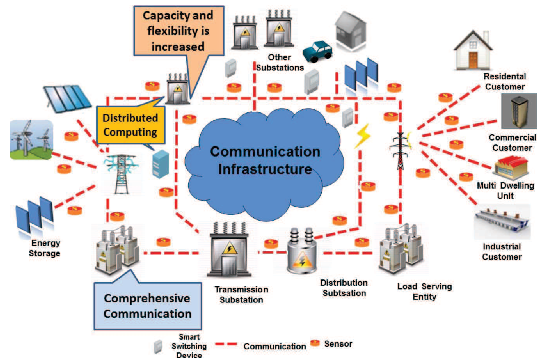
\includegraphics[width=\textwidth]{images/smart-grid-architecture.pdf}
    \caption[Example of a smart energy grid architecture]{A smart energy grid architecture. \cite{gungor-smart-grid-technologies}}
    \label{fig:intro:iot:smart-grid}
\end{figure}

\begin{figure}
    \centering
    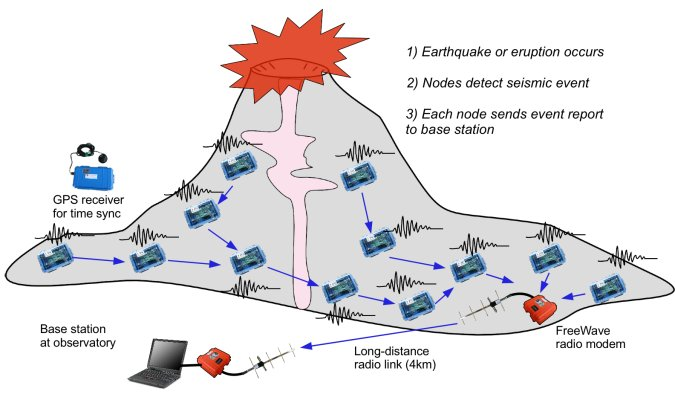
\includegraphics[width=\textwidth]{images/reventador.jpg}
    \caption[Example of IoT deployed on active volcano]{An \gls{IoT} deployed by the Harvard Sensor Networks Lab on an active volcano to monitor seismic activity. \cite{reventador}}
    \label{fig:intro:iot:reventador}
\end{figure}

\subsection{Wireless sensor networks}
\label{sec:intro:wsn}
Many \gls{IoT} applications are implemented using a \acrfull{WSN}. A \gls{WSN} consists of a number of small devices (often called `nodes' or `motes') equipped with sensors, actuators and a wireless antenna. These nodes measure changes in their environment using their sensors, communicate with each other and the outside world using their wireless connectivity and act upon their environment using their actuators.

These nodes have very different characteristics compared to regular computers, and have different design concerns for their programs:
\begin{itemize}
\item Due to their small size, they have extreme resource constraints. Whereas ordinary computers have multi-core \gls{GHz} processors with many \glspl{GB} of RAM, \gls{WSN} nodes have single-core \gls{MHz} microprocessors with only a few \glspl{KB} of RAM. For example, the tiny TMote Sky has a 8 \gls{MHz} microprocessor with 48 \gls{KB} of \gls{RAM} \cite{tmote-sky-manual}, while the larger AVR Zigduino r2 platform runs at 16 \gls{MHz} with 128 \gls{KB} of flash \gls{RAM} \cite{zigduino-manual}.
\item When deployed in remote outside locations (e.g. on a volcano or along a river), they have to be battery-powered or self-provisioning (e.g. small solar panel). This makes energy consumption a primary design concern for programmers, as the node's lifetime is constrained by its battery.
\item Nodes have no infrastructural support: there are no routers or wireless access points to support their communication. All nodes are responsible for sensing their environment, processing their data and routing messages across the network.
\item \gls{WSN} deployments are inherently unreliable. Nodes may fail due to their batteries running out or being destroyed by the environment (e.g. floods, fires or earthquakes). Transmitted messages may be lost due to bad weather conditions. Programmers must design with these failures in mind.
\item \glspl{WSN} are highly distributed. A network may consist of hundreds or thousands of nodes, with nodes moving in and out of range of each other all the time. Distributed programs must be able to scale up to large number of nodes and remain efficient.
\item A single \gls{WSN} may consist of many different types of devices with varying capabilities, specifications and architectures. Programs need to be compiled and configured to work on different device types.
\end{itemize}

\begin{figure}
	\centering
	\begin{subfigure}[b]{.5\textwidth}
		\centering
		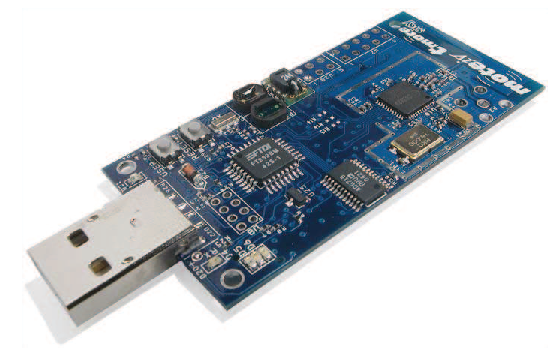
\includegraphics[width=\textwidth]{images/tmote-sky.pdf}
		\caption{The TMote Sky platform.}
		\label{fig:intro:motes:sky}
	\end{subfigure}%
	\begin{subfigure}[b]{.5\textwidth}
		\centering
		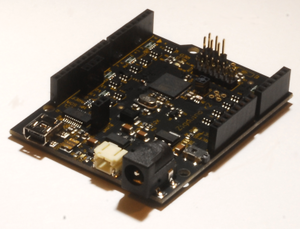
\includegraphics[width=\textwidth]{images/zigduino-r2.png}
		\caption{The AVR Zigduino r2 platform.}
		\label{fig:intro:motes:zigduino}
	\end{subfigure}
	\caption{Sample platforms for WSN motes.}
	\label{fig:intro:motes}
\end{figure}

In order to support wireless \gls{IPv6} connectivity for these low-powered devices, new Internet standards were introduced:
\begin{itemize}
\item \gls{IEEE} 802.15.4 \cite{ieee-802.15.4} specifies the physical network layer and media access control. It focuses on low power and low data rate wireless connectivity among inexpensive devices, as opposed to e.g. Wi-Fi which provides higher data rates but uses significantly more power.
\item \acrfull{6LoWPAN} \cite{rfc6282} allows \gls{IPv6} packets to be sent over \gls{IEEE} 802.15.4 networks. The standard introduces various adaptations to achieve this, such as LoWPAN encapsulation and header compression.
\end{itemize}

To allow access from outside networks, a border router is usually deployed at the edge of the network. The border router translates between \gls{6LoWPAN} packets and standard \gls{IPv6} packets and routes packets between the \gls{WSN} and the rest of the Internet.

\subsection{Peer-to-peer architectures}
\label{sec:intro:p2p}
\Acrfull{P2P} architectures consist of peers with equal capabilities and responsibilities where the work load of the application is distributed over every peer. Peers communicate with each other to retrieve information needed to perform their part of the work, and provide information to other peers to help them with their work. Although peers may different in their resource capacity and processing power, they have the same role in the architecture and can take on the same kinds of tasks.

\Gls{P2P} architectures differ from the more classical client-server architectures, in which a server \emph{provides} resources or services to be \emph{consumed} by one or more requesting clients. Clients and servers are two distinct roles in the architecture with different capabilities responsibilities, and take up distinct parts of the application's work load. For example, the client is not concerned with how the server manages its resources and services, and the server is not concerned with what the client does with the provided resource or service.

Figure \ref{fig:intro:arch} gives an overview of client-server and \gls{P2P} architectures. Figure \ref{fig:intro:arch:client-server} shows multiple clients requesting services from a single server, and figure \ref{fig:intro:arch:p2p} shows many peers communicating to request and provide services among each other. Note that clients in the client-server architecture always communicate with the server and do not communicate directly with each other, whereas peers in the \gls{P2P} architecture can communicate with any other peer.

Many Internet applications use a client-server architecture. For example, the Web consists of web servers providing web pages and web browsers requesting them. Web browsers act as clients and are responsible for sending \gls{HTTP} requests to the appropriate web server and rendering their responses as web pages on the user's screen. Web servers listen for \gls{HTTP} requests and are responsible for producing a response. The web server can do all sorts of processing behind the scenes (e.g. accessing a database) to generate this response, but the client doesn't need to know about any of this and is only concerned with the server's response.

\Acrlong{P2P} applications are less common, but have interesting applications. BitTorrent is a popular \gls{P2P} file sharing protocol, where peers download and upload parts of a file to each other to help distribute the file to all peers (see \ref{sec:related:bittorrent}). Cryptocurrencies such as Bitcoin \footnote{\url{https://bitcoin.org/}} are a fairly recent invention, where peers verify and propagate transactions of a digital currency to ensure that every peer agrees on how much money every user has -- without the need for a centralized authority such as a central bank. In both applications, every peer has the same role in the architecture and can communicate with any other peer.

\begin{figure}
	\centering
	\begin{subfigure}[b]{.5\textwidth}
		\centering
		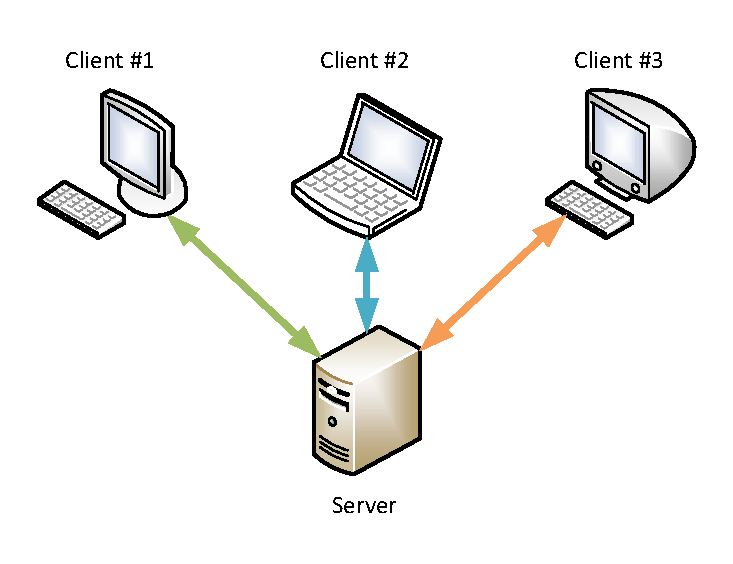
\includegraphics[width=\textwidth]{diagrams/client-server.pdf}
		\caption{Client-server architecture.}
		\label{fig:intro:arch:client-server}
	\end{subfigure}%
	\begin{subfigure}[b]{.5\textwidth}
		\centering
		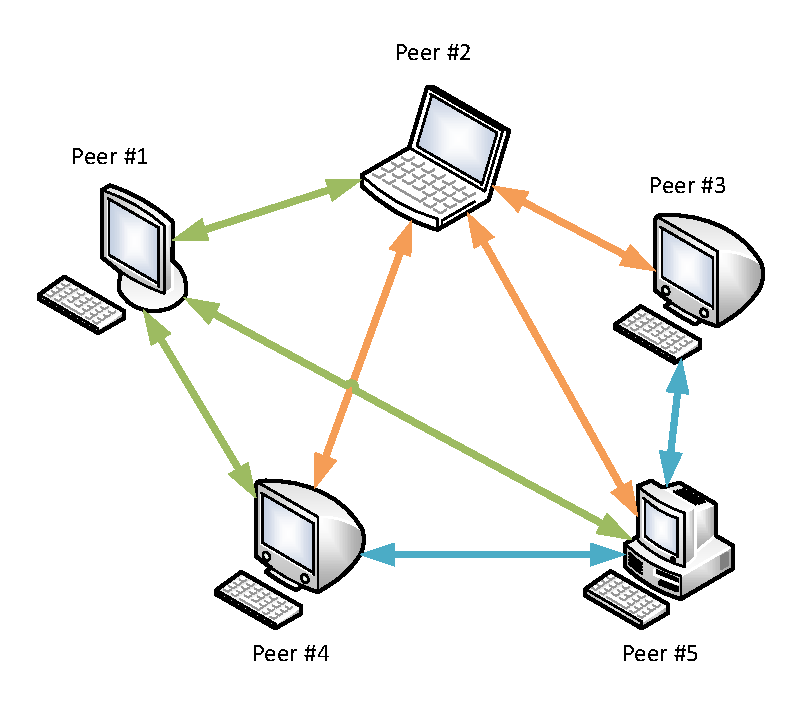
\includegraphics[width=\textwidth]{diagrams/p2p.pdf}
		\caption{Peer-to-peer architecture.}
		\label{fig:intro:arch:p2p}
	\end{subfigure}
	\caption[Server-client and P2P architectural overview]{Overview of server-client and \gls{P2P} architectures.}
	\label{fig:intro:arch}
\end{figure}

\section{Problem description}
\label{sec:intro:problem}
In order to keep \acrlongpl{WSN} operating for long periods of time, they must be able to adapt and evolve even after deployment. Over time, nodes may need to be updated with an updated program binary, a new configuration file or a new data set to be processed. However, it is often not practical and sometimes even impossible to collect a deployed node, take it back to a lab to be reprogrammed with the updated data and then re-deploy it in its original location. Therefore, these updates need to be done `over-the-air': they must be distributed over the \gls{WSN} and received by all destined nodes so these nodes can reconfigure themselves.

For such over-the-air reconfigurations, \gls{WSN} nodes need to be equipped with the proper reconfiguration mechanisms. For example, in the current version (2.0.3) of the LooCI \cite{looci} platform for Contiki \cite{contiki} nodes, the reconfiguration engine is responsible for listening for reconfiguration events, downloading the new program file over \gls{TCP} and reprogramming the node with the downloaded program. This allows LooCI nodes to be completely reprogrammed remotely, without physical intervention. However, this solution is client-server based, with all nodes requesting the download from a single server. When the number of nodes becomes larger, this can put a lot of strain on both the server and the network as many \gls{TCP} connections try to reach this single server. In contrast, a \gls{P2P} approach would balance the load over all the nodes in the network by having them all participate in the program file's distribution. This allows it to be more battery-efficient on the nodes closest to the file's source, and more scalable when the network expands.

This master's thesis focuses on the file distribution mechanism for over-the-air reconfigurations. The objective is to design, implement and evaluate a file distribution protocol optimized for \glspl{WSN}. This protocol could then be used in a complete reconfiguration solution, for example it could replace the \gls{TCP} download in LooCI, allowing for a more efficient program file distribution.

The peculiarities of \acrfullpl{WSN} (discussed in \ref{sec:intro:wsn}) pose many challenges for the design of a file distribution mechanism:
\begin{itemize}
\item File distribution requires large pieces of data to be transmitted in a short time, much larger than usually sent during normal operation of the \gls{WSN}. The transmissions sent between nodes during normal operation most of the time fits in a single packet. This data usually consists of a few measurements, a new average or a notification to the other node -- which all take up only a couple of bytes. However, large files such as programs or configurations do not fit in a single communication packet and cause much more traffic than normal operations. Since most of a node's energy is spent on its antenna and radio, a file distribution mechanism for \glspl{WSN} should be efficient with the amount of packets needed to transmit the whole file in order to save the node's battery.
\item The file should be distributed fast enough to allow nodes to return to their normal operation quickly. While a new program or configuration is propagating through the network, normal operations are largely halted. When nodes cannot be used for their intended purpose for a prolonged period of time, they might miss important measurements or fail to respond to critical events in the environment.
\item Nodes should be able to continue file distribution even when one or more nodes fail, either temporarily or indefinitely. Nodes may need to re-download (a part of) the file and/or use a different route, but a single failure must not take down the whole network. When a failed node comes back online, it should be able to resume the file distribution, preferably without having to restart the download from scratch.
\item Integrity of the distributed file must be guaranteed at every node. The file must be delivered correctly, since any error could corrupt the distributed program or configuration file. Since \glspl{WSN} are unreliable, file distribution mechanisms must be able to verify the received file and recover from transmission errors.
\item The file distribution mechanism must be able to target any subset of nodes in a \gls{WSN}. \glspl{WSN} can be heterogeneous, consisting of different kinds of nodes running different tasks. For example, a \gls{WSN} to measure weather conditions could consist of different nodes to measure temperature, humidity or wind speeds. These nodes have different sensors and run different programs, but can be part of the same network.
\end{itemize}

\section{Contributions}
\label{sec:intro:contrib}
This master's thesis presents NanoTorrent as a possible solution for file distribution in \acrlongpl{WSN}.

NanoTorrent takes a \acrlong{P2P} approach to the problem, where nodes act as peers and download and upload pieces of the file to each other. The design is inspired by the BitTorrent protocol, which has proven to be very successful on the Internet scale. By adopting ideas from BitTorrent, the solution can provide fast distribution speeds to many nodes without the need of an individual high-speed file server. However, it includes many adaptations to take advantages of the unique properties of \glspl{WSN} (discussed in \ref{sec:intro:wsn}) and deal with their challenges (mentioned in \ref{sec:intro:problem})

The main contribution of NanoTorrent is the exploration of a hybrid peer discovery mechanism. BitTorrent mainly uses a tracker for discovering peers, while existing \gls{WSN} distribution protocols only discover directly connected neighbour nodes. NanoTorrent combines both approaches into one solution, where the two mechanisms are used in parallel to connect with both close-by local peers and distant remote peers. This allows NanoTorrent to function in more heterogeneous \gls{WSN} deployments, where not all nodes run the same program or are located on different networks.

The evaluation of the protocol shows that NanoTorrent can provide fast file distribution in many different network configurations. The distribution speed scales well with the size of the network, although in its current form the amount of transmissions is still an issue. The hybrid peer discovery approach means that peers send a lot of messages to discover other peers, and can find distant peers which require messages to take multiple hops across the network to reach them. More research and experimentation is needed to reduce the needed communications.

\section{Structure of the text}
\label{sec:intro:structure}

\begin{itemize}

\item Chapter \ref{cha:intro} is an introduction to the problem context of \gls{IoT} and the challenges posed by file distribution for \glspl{WSN}. It outlines the contributions of this master's thesis.

\item Chapter \ref{cha:related-work} discusses the researched related work regarding \gls{P2P} protocols on the Internet and in \glspl{WSN}.

\item Chapter \ref{cha:discovery} introduces the first half of NanoTorrent's protocol design, with the hybrid peer discovery mechanism. It describes both the centralized approach with a tracker managing the swarm, and the localized approach using link-local multicast announcements.

\item Chapter \ref{cha:distribution} gives the other half of the protocol design, focusing on the file distribution aspect. It discusses the different parts of the protocol, such as how peers connect with each other, how they exchange pieces and how it takes advantage of locality.

\item Chapter \ref{cha:implementation} explains the technicalities of the create prototype implementation. It describes the system architecture and its components such as the tracker, the border router and the peers.

\item Chapter \ref{cha:evaluation} discusses the evaluation of the protocol design and the prototype implementation. Experiments were performed in a simulated environment to analyse the scalability of the protocol, and its operation in a heterogeneous network.

\item Chapter \ref{cha:conclusion} concludes the text with a summary of all chapters, the lessons learned in making this thesis and possible future work building on this thesis.

\end{itemize}